\documentclass[]{beamer}
\usepackage{mathptmx}
\usepackage{graphicx}
\usepackage{parskip}
\usepackage{verbatim}
\usepackage{listings}
\usepackage{dtsyntax}
\usepackage[english]{babel}
\usepackage[utf8]{inputenc}
\usepackage{booktabs}
\usepackage{float}
\usepackage{ulem}
\usepackage{color}
\usepackage{multirow}
\usepackage{lipsum}
\usepackage{epstopdf}
\usepackage{bm}

\newcommand\gsout{\bgroup\markoverwith
{\textcolor{green}{\rule[3.1pt]{2pt}{1pt}}}\ULon}

%%%%%%%%%% Regler Beamer themes %%%%%%%%%%%%%%%%%
%\usepackage[lionbackground]{beamerthemeRegler}
%\usepackage[lioncorner]{beamerthemeRegler}
%\usepackage[lionheader]{beamerthemeRegler}
\usetheme[lionheader]{Regler}
%%%%%%%%%%%%%%%%%%%%%%%%%%%%%%%%%%%%%%%%%%%%%%%%%

% Title page
\title{Implicit vs. explicit ODE}
\author{Fredrik Magnusson\inst{1} \and Karl Berntorp\inst{2} \\ Christan \& Claus?}
\institute
{
\inst{1} Department of Automatic Control \\
Lund University, Sweden \\
\vspace{14pt}
\inst{2} Mitsubishi Electric Research Laboratories \\
Cambridge, MA \\
\vspace{14pt}
\insertdate
}
\date{October 15, 2015}


% Slide numbering
\definecolor{FootGrey}{RGB}{83,121,170}
\setbeamercolor{foot}{fg=FootGrey,bg=white}
\setbeamertemplate{footline}{
    \begin{beamercolorbox}[right, sep=2.5pt]{foot}
        \insertframenumber{} / \inserttotalframenumber
    \end{beamercolorbox}
}

\begin{document}

{
\setbeamertemplate{footline}{}
\begin{frame}[noframenumbering]
    \titlepage
\end{frame}
}

\begin{frame}
\frametitle{Review}
Last time:
\begin{itemize}
\item
Compared simulation results for implicit DAE and explicit ODE with IDA and Radau5
\item
Implicit DAE formulation needs 10-20 times more steps
\item
Suppressing algebraic variables behaves very similarly to explicit ODE
\item
Pacejka Magic Formula (algebraic equation) stiff
\item
Surprisingly large relative errors with ODE formulation
\end{itemize}
\end{frame}

\begin{frame}
\frametitle{Preview}
This time:
\begin{itemize}
\item
Revisit the error comparisons
\item
Discuss how all of this affects optimization
\end{itemize}
\end{frame}

\begin{frame}
\frametitle{Partial DAE}
\begin{itemize}
\item
Last time considered eliminating all algebraics except the 4 nominal forces (Magic formula)
\item
I tested this as well, and call it DAE par.
\end{itemize}
\end{frame}

\begin{frame}
\frametitle{Simulation results}
Radau5 tolerance chosen to get reference solution, the rest to get similar accuracy

\begin{table}
\centering
\begin{tabular}{lcccc}
\toprule
Setup & tol & Time [s] & Steps [1000] & Evals [1000] \\
\midrule
Radau5 DAE & 1e-12 & 69 & 17 & 640 \\
IDA DAE & 1e-6 & 59 & 26 & 930 \\
IDA DAE sup. alg. & 1e-8 & 2.8 & 2.9 & 42 \\
IDA DAE par. & 1e-6 & 6.3 & 8 & 102 \\
IDA ODE & 1e-8 & 0.9 & 3.4 & 15 \\
\bottomrule
\end{tabular}
\end{table}
\end{frame}

\begin{frame}[fragile]
\frametitle{Radau5 DAE}
{\small
\begin{verbatim}
Final Run Statistics: --- 

 Number of steps                                 : 16701
 Number of function evaluations                  : 231074
 Number of Jacobian evaluations                  : 12338
 Number of function eval. due to Jacobian eval.  : 407154
 Number of error test failures                   : 1040
 Number of LU decompositions                     : 21266

Solver options:

 Solver                  : Radau5 (implicit)
 Tolerances (absolute)   : [  1.00000000e-12]
 Tolerances (relative)   : 1e-12
\end{verbatim}
}
\end{frame}

\begin{frame}[fragile]
\frametitle{IDA DAE}
{\small
\begin{verbatim}
Final Run Statistics: --- 

 Number of steps                                 : 26361
 Number of function evaluations                  : 67823
 Number of Jacobian evaluations                  : 25991
 Number of function eval. due to Jacobian eval.  : 857703
 Number of error test failures                   : 12046
 Number of nonlinear iterations                  : 67823
 Number of nonlinear convergence failures        : 0

Solver options:

 Solver                       : IDA (BDF)
 Maximal order                : 5
 Suppressed algebr. variables : False
 Tolerances (absolute)        : 1e-06
 Tolerances (relative)        : 1e-06
\end{verbatim}
}
\end{frame}

\begin{frame}[fragile]
\frametitle{IDA DAE sup. alg.}
{\small
\begin{verbatim}
Final Run Statistics: --- 

 Number of steps                                 : 2923
 Number of function evaluations                  : 7072
 Number of Jacobian evaluations                  : 1065
 Number of function eval. due to Jacobian eval.  : 35145
 Number of error test failures                   : 424
 Number of nonlinear iterations                  : 7072
 Number of nonlinear convergence failures        : 0

Solver options:

 Solver                       : IDA (BDF)
 Maximal order                : 5
 Suppressed algebr. variables : True
 Tolerances (absolute)        : 1e-08
 Tolerances (relative)        : 1e-08
\end{verbatim}
}
\end{frame}

\begin{frame}[fragile]
\frametitle{IDA DAE par.}
{\small
\begin{verbatim}
Final Run Statistics: --- 

 Number of steps                                 : 8489
 Number of function evaluations                  : 18467
 Number of Jacobian evaluations                  : 5952
 Number of function eval. due to Jacobian eval.  : 83328
 Number of error test failures                   : 2867
 Number of nonlinear iterations                  : 18467
 Number of nonlinear convergence failures        : 0

Solver options:

 Solver                       : IDA (BDF)
 Maximal order                : 5
 Suppressed algebr. variables : False
 Tolerances (absolute)        : 1e-06
 Tolerances (relative)        : 1e-06
\end{verbatim}
}
\end{frame}

\begin{frame}[fragile]
\frametitle{IDA ODE}
{\small
\begin{verbatim}
Final Run Statistics: --- 

 Number of steps                                 : 3428
 Number of function evaluations                  : 5524
 Number of Jacobian evaluations                  : 919
 Number of function eval. due to Jacobian eval.  : 9190
 Number of error test failures                   : 477
 Number of nonlinear iterations                  : 5524
 Number of nonlinear convergence failures        : 0

Solver options:

 Solver                       : IDA (BDF)
 Maximal order                : 5
 Suppressed algebr. variables : False
 Tolerances (absolute)        : 1e-08
 Tolerances (relative)        : 1e-08
\end{verbatim}
}
\end{frame}

\begin{frame}[fragile]
\frametitle{Error}
\begin{itemize}
\item
Reference solution $v$ from Radau5 with \verb|ATOL=RTOL=1e-12|
\item
Compare with the various IDA solutions $\hat v$, all with \verb|ATOL=RTOL=1e-6|
\item
Compute relative error as function of time for each variable kind:
\[e_v(t) = \left|\left|\frac{v(t) - \hat v(t)}{v(t) + \epsilon_{\text{mach}}}\right|\right|_\infty, \quad \forall v \in \{\dot x, x, y\}\]
\end{itemize}
\end{frame}

\begin{frame}
\frametitle{Variable kind errors}
\begin{figure}[ht]
\centering
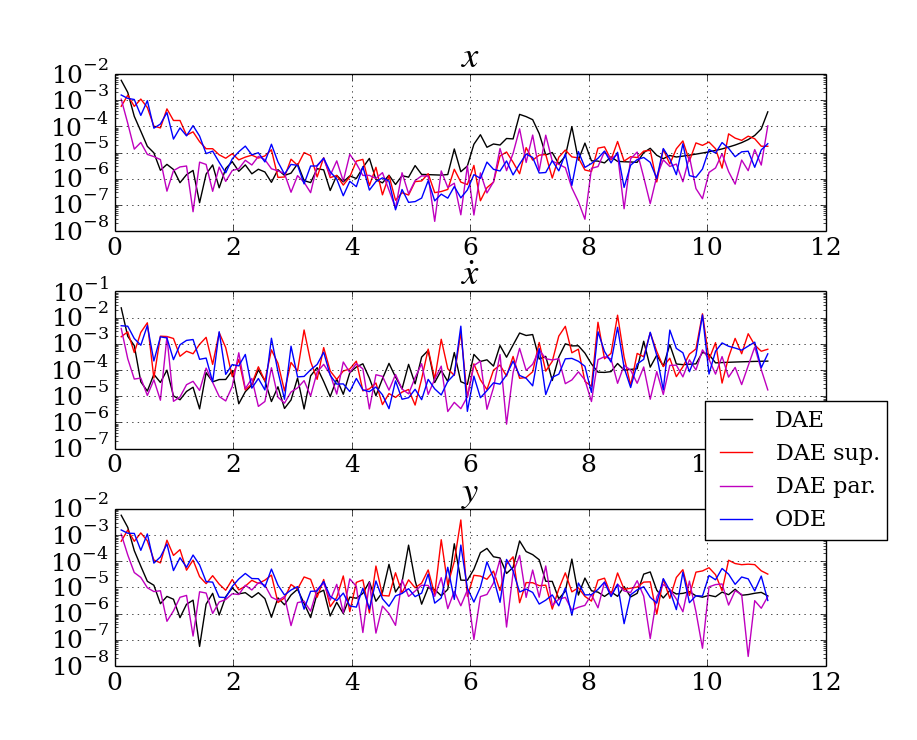
\includegraphics[width=0.9\linewidth]{errors.png}
\end{figure}
\end{frame}

\begin{frame}
\frametitle{Variable kind errors}
Can we conclude that ODE formulation is superior for simulation?
\end{frame}

\begin{frame}
\frametitle{Commutativity}
\begin{itemize}
\item
Last time: Does BLT and fixed-step collocation commute?
\item
Consider single integration step of
\begin{equation}
\begin{aligned}
\dot x &= f(x, y, u) \\
y &= g(x, u),
\end{aligned}
\end{equation}
and
\begin{equation}
\dot x = f(x, g(x, u), u)
\end{equation}
\end{itemize}
\end{frame}

\begin{frame}
\frametitle{Commutativity}
Explicit DAE:
\begin{subequations}
\begin{gather}
\dot x_k = f(x_k, y_k, u_k), \\ 
y_k = g(x_k, u_k), \\
\dot{x}_k = \frac{1}{h} \cdot \sum_{n = 0}^{n_c} \alpha_{n, k} x_n, \\
\forall k \in [1 . . n_c]
\end{gather} 
\end{subequations}

Explicit ODE:
\begin{subequations}
\begin{gather}
\dot x_k = f(x_k, g(x_k, u_k), u_k), \\ 
\dot{x}_k = \frac{1}{h} \cdot \sum_{n = 0}^{n_c} \alpha_{n, k} x_n, \\
\forall k \in [1 . . n_c]
\end{gather} 
\end{subequations}

Clearly commutative?
\end{frame}

\begin{frame}
\frametitle{Dynamic optimization}
{\small
\begin{subequations}\label{eq:DOP}
\begin{alignat}{3}
& \text{minimize \hspace{10pt}} && \rlap{$\phi(t_0, t_f, \bm z_T, \bm p) + \displaystyle\int_{t_0}^{t_f} L(t, \bm z(t), \bm z_T, \bm p)\,\mathrm{d}t \label{eq:DOP!objective}$} && \\
& \text{with respect to \hspace{10pt}} && \rlap{$\bm x : [t_0, t_f] \rightarrow \mathbb{R}^{n_x}, \quad \bm y : [t_0, t_f] \rightarrow \mathbb{R}^{n_y}, \quad \bm u : [t_0, t_f] \rightarrow \mathbb{R}^{n_u} \nonumber$}  &\quad& \hspace{170pt} \\
&&& t_0 \in \mathbb{R}, \quad t_f \in \mathbb{R}, \quad \bm p \in \mathbb{R}^{n_p} && \nonumber \\
& \text{subject to \hspace{10pt}} && \bm F(t, \bm z(t), \bm p) = \bm 0, &\quad& \bm F_0(t_0, \bm z(t_0), \bm p) = \bm 0 \label{eq:DOP!dynamics}\\
&&& \bm z_L \leq \bm z(t) \leq \bm z_U, &\quad& \bm p_L \leq \bm p \leq \bm p_U \label{eq:DOP!bounds} \\
&&& \bm g_e(t_0, t_f, t, \bm z(t), \bm z_T, \bm p) = \bm 0, &\quad& \bm g_i(t_0, t_f, t, \bm z(t), \bm z_T, \bm p) \leq \bm 0 \label{eq:DOP!path_constraints} \\
&&& \bm G_e(t_0, t_f, \bm z_T, \bm p) = \bm 0, &\quad& \bm G_i(t_0, t_f, \bm z_T, \bm p) \leq \bm 0 \label{eq:DOP!point_constraints} \\
&&& \forall t \in [t_0, t_f] && \nonumber
\end{alignat}
\end{subequations}
}
\end{frame}

\end{document} 
